% (c) 2010 Konstantin Sering <konstantin.sering <aet> gmail.com>
% (cc)-by -- Licenced under Creative Commons Attribution unported
% (http://creativecommons.org/licenses/by/3.0/)
%
\documentclass[xcolor={fixpdftex,hyperref,x11names},10pt,pdftex,hyperref={pdftex}]{beamer}
 
% Pakete
\usepackage[utf8]{inputenc}
\usepackage{lmodern}
\usepackage[T1]{fontenc}
\usepackage[english]{babel}
\usepackage{graphicx}
\usepackage{booktabs}
\usepackage{amssymb}
\usepackage{amsmath}
\usepackage{tikz}
\usepackage{fancyvrb}
\usepackage{color}
%\usepackage{apacite}
\usepackage{amsmath}
%\usepackage{txfonts}
%\usepackage{showframe}
%\useoutertheme{tree}
\useinnertheme{circles}
\usecolortheme{orchid}
\usecolortheme{whale}
%\usecolortheme{blue}
\usefonttheme[onlymath]{serif}
\usetikzlibrary{arrows,shapes}


% Informationen
\title{Applying IICM to simulated 3D IDM}
\subtitle{ESMP 2013 -- Group 7}
\author{Micha, Michael, Marilisa, Jan, and Tino}
\institute{European Union -- Oulanka Research Station}
\date{23.03.2013}

\setbeamertemplate{navigation symbols}{} 
\setbeamertemplate{footline}{\hspace*{.5cm}\small{\hspace*{50pt} 
\hfill\insertframenumber/\inserttotalframenumber\hspace*{.5cm}}} 
%\setbeamertemplate{headline}{} % removes the headline that infolines inserts

% Sonstiges
\renewcommand{\emph}[1]{\color{red}#1 \color{black}}

\begin{document}

\maketitle

\section{Motivation}
\label{sec:motivation}



\begin{frame}
  \frametitle{Goal}
  \begin{columns}
  \begin{column}{0.30\textwidth}
  
\includegraphics[width=0.7\textwidth]{figs/checkbox-unchecked.png}
  \end{column}
  \begin{column}{0.70\textwidth}
  With an extended IDM model, simulate human behaviour in a three-alternative temporal judgment task
  \end{column}
  \end{columns}
  \begin{columns}
  \begin{column}{0.30\textwidth}
  
\includegraphics[width=0.7\textwidth]{figs/checkbox-unchecked.png}
  \end{column}
  \begin{column}{0.70\textwidth}
  Fit Independent-Channels Model (Miguel \& Rocio) to our simulated data 
  \end{column}
  \end{columns}
\end{frame} 




%%%%%%%%%%%%%%%%%%%%%%%%%%%
\section{Temporal Judgment Tasks}
\label{sec:tjt}
%\section{Decision Tasks}

\begin{frame}
	\frametitle{General Idea}

	\begin{itemize}
		\item Observer's ability to elucidate whether two sensory stimuli occured simultaneously or not.
		\item measured as a function of stimulus onset asychnchrony (SOA)
		\item[$\rightarrow$] here audiovisual case (visual regarded as reference)
		\item independent variable is auditory delay

	\end{itemize}
	
\begin{center}
% nice picture of SOA
	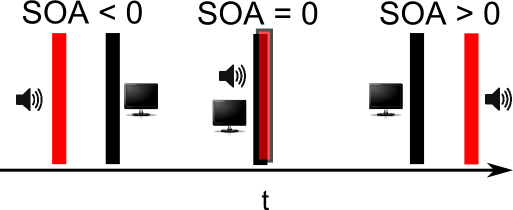
\includegraphics[width=0.7\textwidth]{figs/SOA-in-task.png}
\end{center}
	
%%%%%%%%%%%%%%%%%%%%%%%%%%%%%
\end{frame}


\begin{frame}
	\frametitle{Synchrony judgment (SJ)}

	\begin{itemize}
		\item Three possible repsonses (SJ3):
			\begin{enumerate}
				\item \textit{audio-first} (AF)
				\item \textit{video-first} (VF)
				\item \textit{synchronous} (S)
			\end{enumerate}

		\item[$\rightarrow$] Psychometric function: proportion of responses of
		 each type as a function of auditory delay.

	\end{itemize}
	

	\begin{center}
		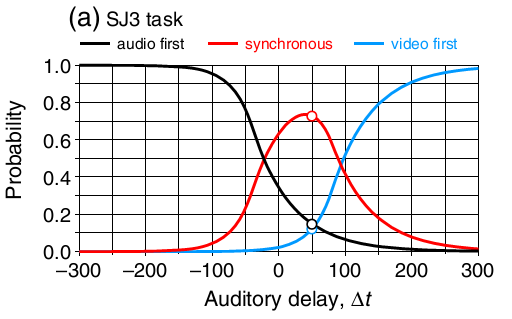
\includegraphics[width=0.7\textwidth]{figs/SJ3-psychometric-function.png}
	\end{center}
\end{frame}


%%%%%%%%%%%%%%%%%%%%%%%%%%%%%

%\begin{frame}
%	\frametitle{Quantitative Indices}

%	\begin{itemize}
%		\item Two quantitative indices obtain from such tasks
%			\begin{enumerate}
%				\item \textit{Point of subjective simultaneity}: midpoint of the synchrony interval. \textit{AF} and \textit{VF} are equally frequent.
%				\item \textit{synchrony range}: width of interval of \textit{S}-responses  (important for simulation)
%			\end{enumerate}

%	\end{itemize}
%	
%%	\begin{center}
%%		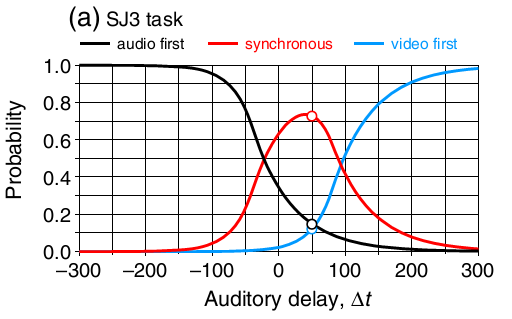
\includegraphics[width=0.7\textwidth]{figs/SJ3-psychometric-function.png}
%%	\end{center}

%\end{frame}



%%%%%%%%%%%%%%%%%%%%%%%%%%%%%

\section{Ising Decision Making (IDM)}
\label{sec:idm}

\begin{frame}
	\frametitle{Recap on 2D IDM}

\begin{columns}
        \column{.5\textwidth}
	\begin{itemize}
		\item Two pools of $N_p$ neurons
		\item All thresholds $\Theta$
		\item Internal excitation: $ w_{p}^{+} > 0$
		\item Mutual inhibition: $ - w_{12}^2 < 0$
		\item External exciting fields $ b_p > 0 $	
		\item Energy function: 
	\end{itemize}
        \column{.5\textwidth}
                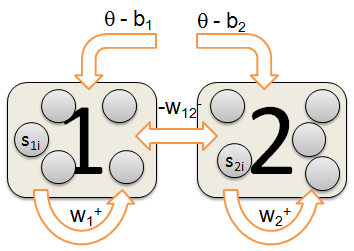
\includegraphics[width=0.99\textwidth]{figs/2D-IDM.png}
\end{columns}


\begin{equation}
\begin{split}
E_{IDM}(S) = &-w_1^{+} \sum_{i<j} S_{1i} S_{1j} - w_2^{+} \sum_{i<j} S_{2i} S_{2j} + w_{12}^{-} \sum_{i,j} S_{1i} S_{2j} \\
&-(b_1 - \Theta) \sum_{i} S_{1i} - (b_1 - \Theta) \sum_{i} S_{2i}
\end{split}
\end{equation}
	
\end{frame}

%%%%%%%%%%%%%%%%%%%%%%%%%%%%%%%
\begin{frame}
	\frametitle{Recap on 2D IDM}

	\begin{itemize}
		\item From Energy Function $E_{IDM}(S)$ to Free Energy Function $F_{IDM}(y)$ with $y_p = \frac{\sum\nolimits_{i} S_{pi}}{N_p}$
	\end{itemize}


\begin{equation}
\begin{split}
F_{IDM}(y) = &-W^{+} + y_1^2 - W^+ y_1 y_2 - (B_1 - \Theta) y_1 - (B_2 - \Theta) y_2 \\
&+ \beta^{-1} \frac{N}{2}\sum_{p} (y_p \log (y_p) + (1-y_p) \log(1-y_p))
\end{split}
\end{equation}

\end{frame}


%%%%%%%%%%%%%%%%%%%%%%%%%%%%%

\begin{frame}
	\frametitle{Recap on 2D IDM}

\begin{columns}
        \column{.5\textwidth}
		Clear Stimulus
	\begin{center}
		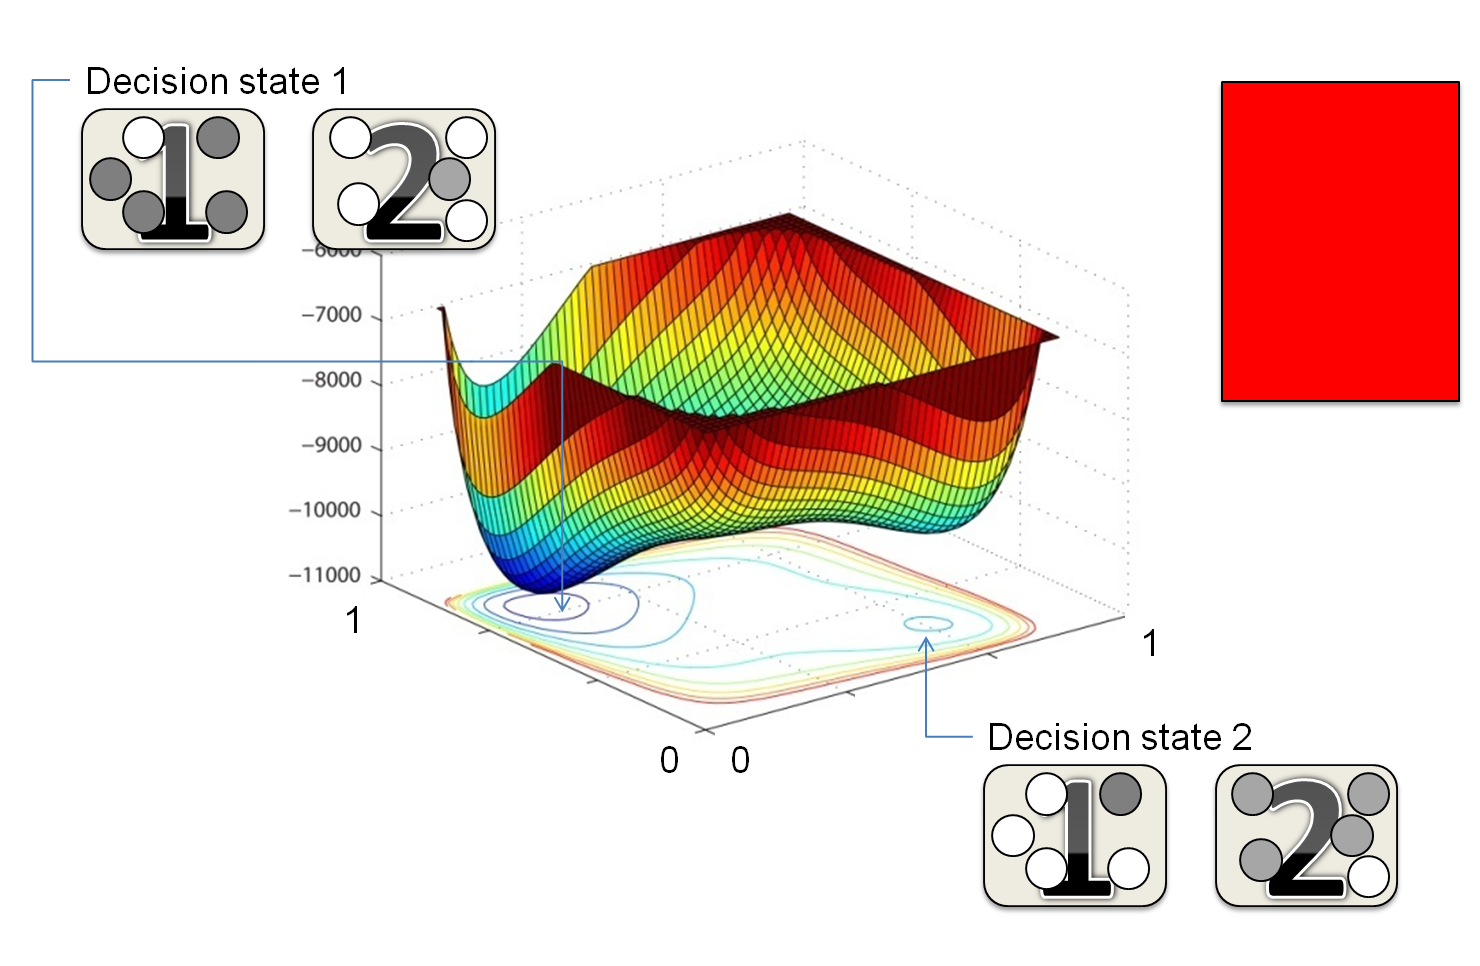
\includegraphics[width=0.99\textwidth]{figs/clear-stim.png}
	\end{center}

        \column{.5\textwidth}
		Unclear Stimulus
    		\begin{center}
			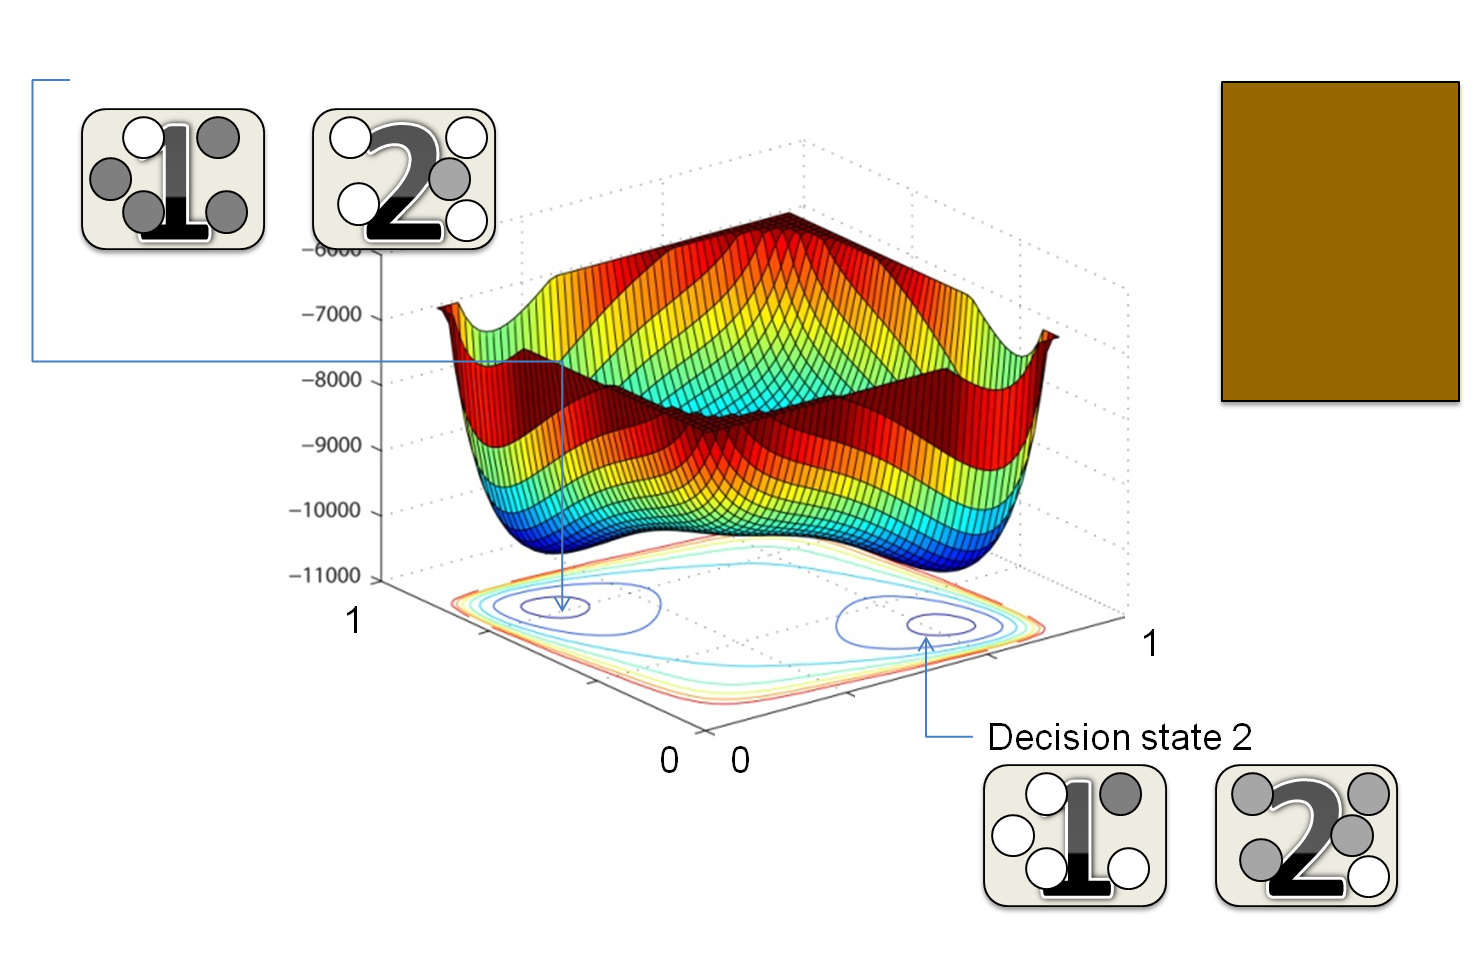
\includegraphics[width=0.99\textwidth]{figs/unclear-stim.png}
		\end{center}

\end{columns}

\end{frame}

%%%%%%%%%%%%%%%%%%%%%%%%%%%%%

\begin{frame}
	\frametitle{Recap on 2D IDM}
One trial
    		\begin{center}
			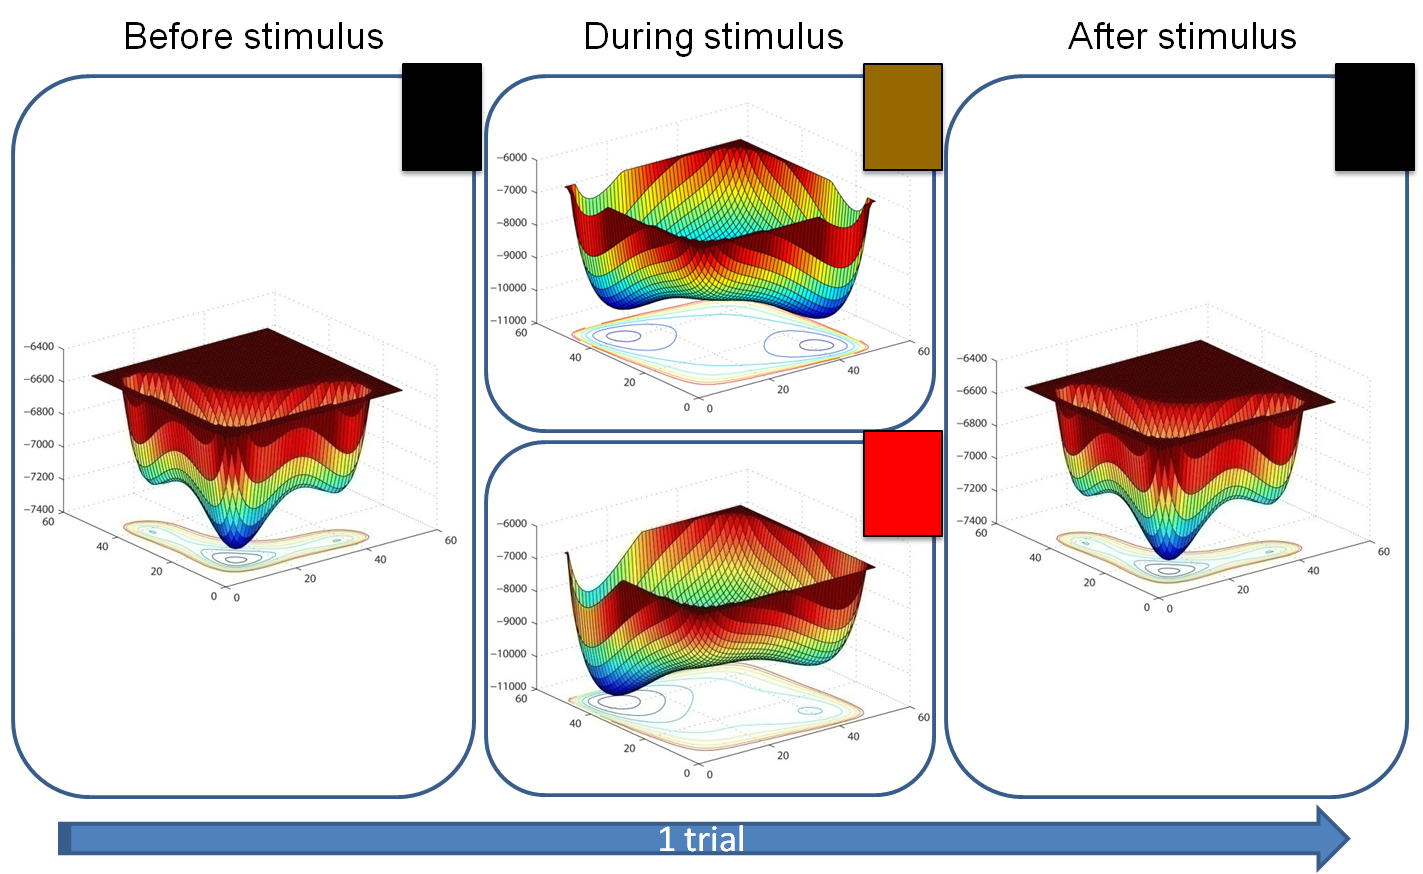
\includegraphics[width=0.99\textwidth]{figs/surface-trial.png}
		\end{center}

\end{frame}

%%%%%%%%%%%%%%%%%%%%%%%%%%%%

\begin{frame}
	\frametitle{Recap on 2D IDM}
Traces
    		\begin{center}
			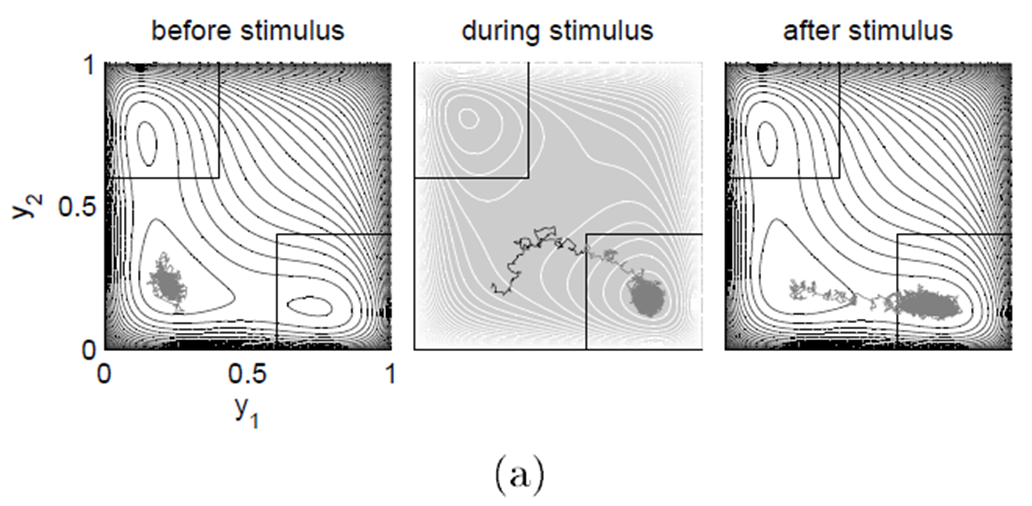
\includegraphics[width=0.99\textwidth]{figs/2D-trace.png}
		\end{center}

\end{frame}

%%%%%%%%%%%%%%%%%%%%%%%%


\begin{frame}
  \frametitle{Goal}
  \begin{columns}
  \begin{column}{0.30\textwidth}
  
\includegraphics[width=0.7\textwidth]{figs/checkbox-unchecked.png}
  \end{column}
  \begin{column}{0.70\textwidth}
  With an extended IDM model, simulate human behaviour in a three-alternative temporal judgment task
  \end{column}
  \end{columns}
  \begin{columns}
  \begin{column}{0.30\textwidth}
  
\includegraphics[width=0.7\textwidth]{figs/checkbox-unchecked.png}
  \end{column}
  \begin{column}{0.70\textwidth}
  Fit Independent-Channels Model (Miguel \& Rocio) to our simulated data 
  \end{column}
  \end{columns}
\end{frame} 
%%%%%%%%%%%%%%%%%%%%%%%%%%%

% tino

%%%%%%%%%%%%%%%%%%%%%%%%%%%%
\begin{frame}
  \frametitle{Goal}
  \begin{columns}
  \begin{column}{0.30\textwidth}
  
\includegraphics[width=0.7\textwidth]{figs/checkbox-checked.png}
  \end{column}
  \begin{column}{0.70\textwidth}
  With an extended IDM model, simulate human behaviour in a three-alternative temporal judgment task
  \end{column}
  \end{columns}
  \begin{columns}
  \begin{column}{0.30\textwidth}
  
\includegraphics[width=0.7\textwidth]{figs/checkbox-unchecked.png}
  \end{column}
  \begin{column}{0.70\textwidth}
  Fit Independent-Channels Model (Miguel \& Rocio) to our simulated data 
  \end{column}
  \end{columns}
\end{frame} 


\section{Simulations}
\label{sec:simu}




\section{Integrated Independent-Channels Model (ICM)}
\label{sec:icm}

\begin{frame}
  \frametitle{Integrated Independent-Channels Model (ICM)}
  \begin{itemize}
   \item  Model distinction between unobservable judgments and 
   observed responses; extension to different time judgment tasks (SJ2, SJ3, TOJ).  
   \item  Signals from 2 stimuli arrive at a central mechanism with 2
    exponentially distributed arrival latencies T1 and T2.
   \newline
  \begin{equation}
   g_i(t) = \lambda_i \text{exp}[-\lambda_i(t-(\Delta t_i + \tau_i ))],
   \quad t \leq \Delta t_i + \tau_i,\quad  i\in\{v,a\}        				                                                                                                                                                                                                                                                                                                                                                                
  \end{equation}
   \newline
   $\mu = \frac{1}{\lambda_i+\tau_i},\quad\sigma = \frac{1}{\lambda_i},
   \quad \Delta t_v=0, \quad\Delta t\equiv\Delta t_a (SOA) $
   \newline
   \item  Judgment of temporal order or synchrony is determined by 
   a ternary decision rule applied to the arrival time 
   difference $D=T_a-T_v$ between the 2 signals.
 \end{itemize}
\end{frame}

\subsection{Model parameters}

\begin{frame}
\frametitle{ICM - Model parameters (1)}
 \begin{columns}[t]
  \begin{column}{0.50\textwidth}
   \begin{figure}[h]
      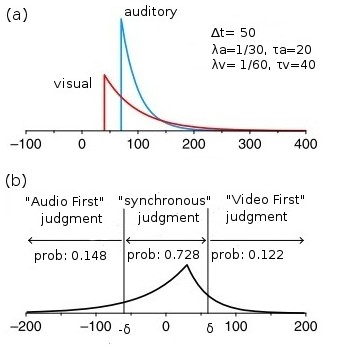
\includegraphics[width=50mm]{figs/SJ3_Figure1.jpg}
      \caption{a) Arrival latency distribution at $T_i$; 
      b) Arrival-time differences distribution $D=T_a-T_v$}
    \end{figure}
  \end{column}
  \begin{column}{0.50\textwidth}
    \vfill
    Resolution parameter $\delta$ (in msec) describes the 
    observer's ability to resolve small differences in arrival 
    latency and defines two cutpoints in the decision space. 
    
    \begin{equation*}
    \begin{array}{l l l}
    D<-\delta & \Rightarrow & \text {AF judgment}\\
    -\delta\leq D\leq\delta & \Rightarrow & \text {S judgment}\\
    D < \delta & \Rightarrow & \text {VF judgment} 
    \end{array}
    \end{equation*}
  \end{column}
 \end{columns}
\end{frame}


\begin{frame}
 \frametitle{ICM - Model parameters (2)}
  Probability of each judgment as a function of auditory delay $\Delta t$ and resolution parameter $\delta$.
  \begin{equation}
   \begin{array}{l}
    \Psi_\text{SJ3 AF}(\Delta t)=\int_{-\delta}^{-\infty} f(z;\Delta t)dz=F(-\delta;\Delta t)\\
    \Psi_\text{SJ3 S}(\Delta t)=\int_{\delta}^{-\delta} f(z;\Delta t)dz=F(\delta;\Delta t)-F(-\delta;\Delta t)\\
    \Psi_\text{SJ3 VF}(\Delta t)=\int_{\infty}^{\delta} f(z;\Delta t)dz=1-F(\delta;\Delta t)
   \end{array}
  \end{equation}
  \begin{figure}[ht!]
   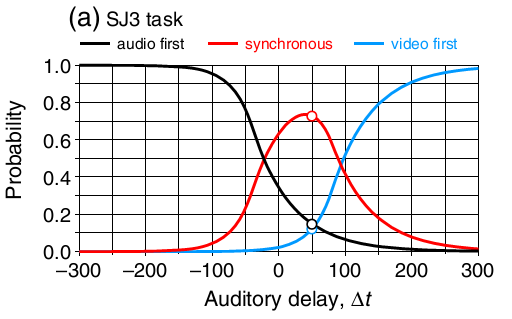
\includegraphics[width=65mm,totalheight=0.5\textheight]{figs/SJ3-psychometric-function.png}
  \end{figure}
\end{frame}


\begin{frame}
  \frametitle{ICM - Model parameters (3)}
   \begin{columns}[t]
    \begin{column}{0.50\textwidth}
    \begin{figure}[h]
      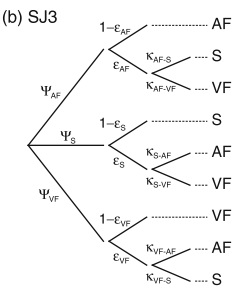
\includegraphics[width=50mm]{figs/SJ3_Figure3.jpg}
    \end{figure}
   \end{column}
  \begin{column}{0.50\textwidth}
   \vfill
   $\varepsilon_\text{AF,S,VF}$ accounts for the probability of 
   judgment misreports according to a response bias $K_\text{X-Y}$ which 
   describes the bias toward misreporting a response Y rather than Z $(1-K_\text{X-Z})$ to the judgment X.  
  \end{column}
 \end{columns}
\end{frame}


\subsection{ICM fit to real data}

\begin{frame}
  \frametitle{ICM - Fit to empirical data}
  Fitted ICM model to four subjects' real data: response proportion
  as a function of auditory delay (SOA)
   \begin{figure}[h]
      \begin{tabular}{c c}
      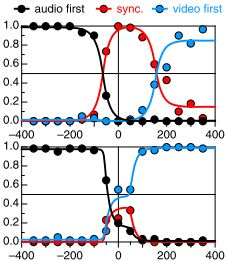
\includegraphics[width=45mm,totalheight=0.4\textheight]{figs/SJ3_Figure4a.jpg}
      &
      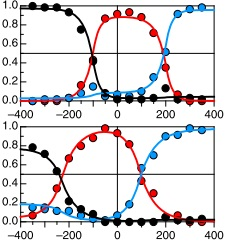
\includegraphics[width=45mm,totalheight=0.4\textheight]{figs/SJ3_Figure4b.jpg}
       \end{tabular}
   \end{figure}
\end{frame} 


\subsection{Fitting ICM to 3D IDM data}

\begin{frame}
  \frametitle{Fitting ICM to 3D IDM data}
  Fitting of ICM model to SJ3 data simulated via 3D IDM: 
  \begin{itemize}
   \item 3 different observers (2 normal and one particularly "skilled")
   \item 216 trials for each of 15 auditory delays ranging from -350 to 350 (steps of 50 msec)
   \item fit of the ICM full model for SJ3 task with error 
   parameters $\varepsilon_\text{AF,S,VF}$ and all different Ks 
  \end{itemize}
\end{frame}


\begin{frame}
  \frametitle{Fitting ICM to 3D IDM data: results (1)}
   \begin{figure}[h]
      \begin{tabular}{c c}
      Left & Right\\
      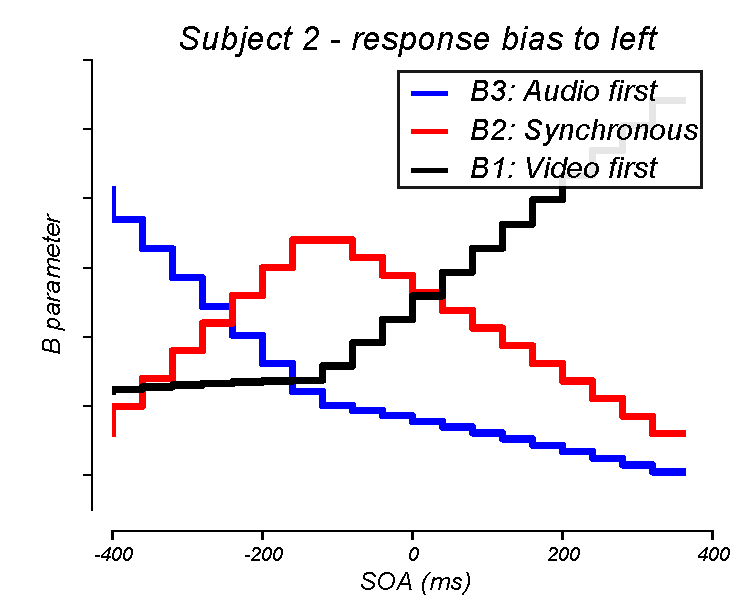
\includegraphics[width=45mm,totalheight=0.4\textheight]{figs/sub2_plot_Bs}
      &
      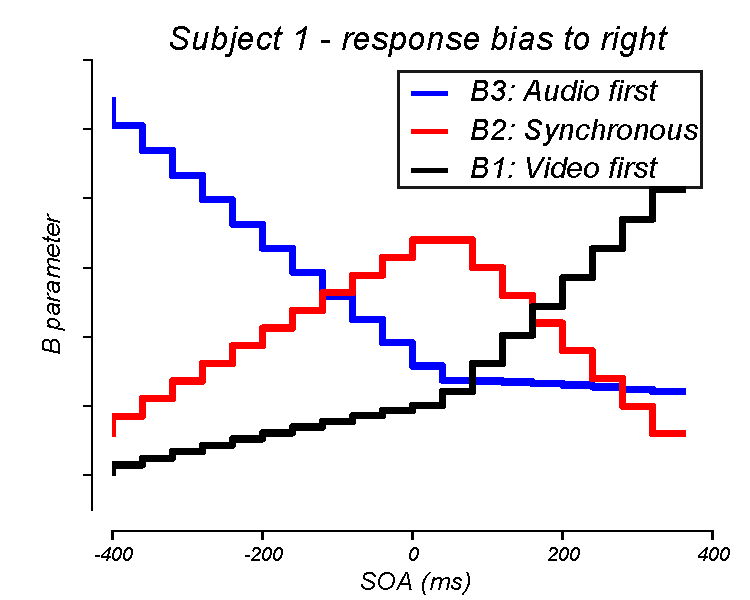
\includegraphics[width=45mm,totalheight=0.4\textheight]{figs/sub1_plot_Bs}\\
        
      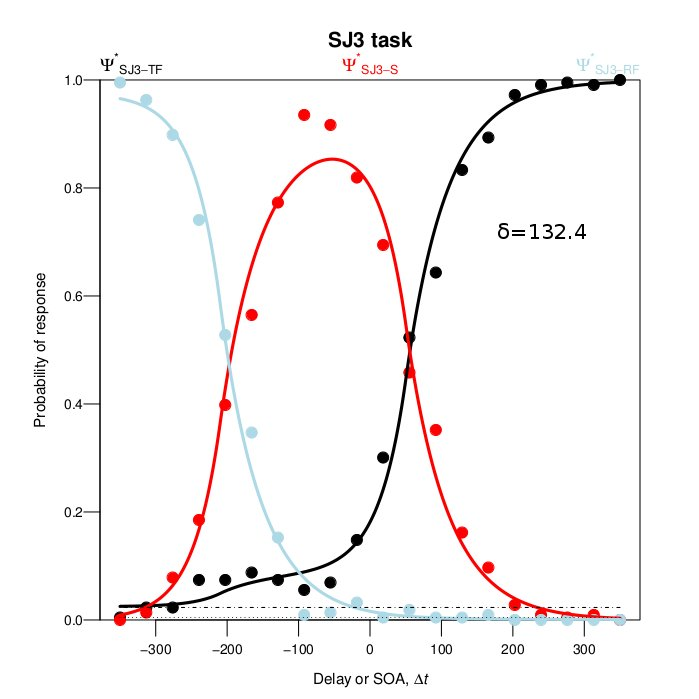
\includegraphics[width=45mm,totalheight=0.4\textheight]{figs/sub2_fitted_model.jpg}
      &
      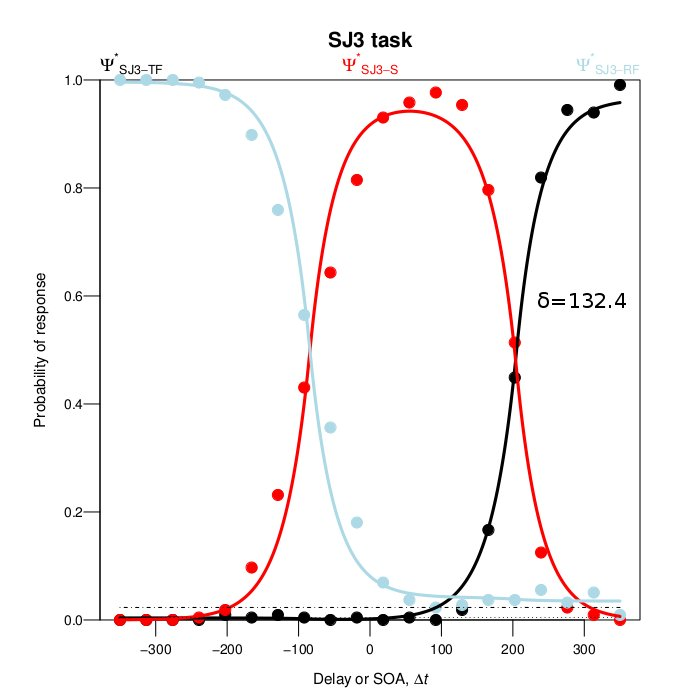
\includegraphics[width=45mm,totalheight=0.4\textheight]{figs/sub1_fitted_model.jpg}
       \end{tabular}
   \end{figure}
\end{frame}  

\begin{frame}
  \frametitle{Fitting ICM to 3D IDM data}
   \centering{A.W.E.S.O.M.O}
   \begin{figure}[h]
    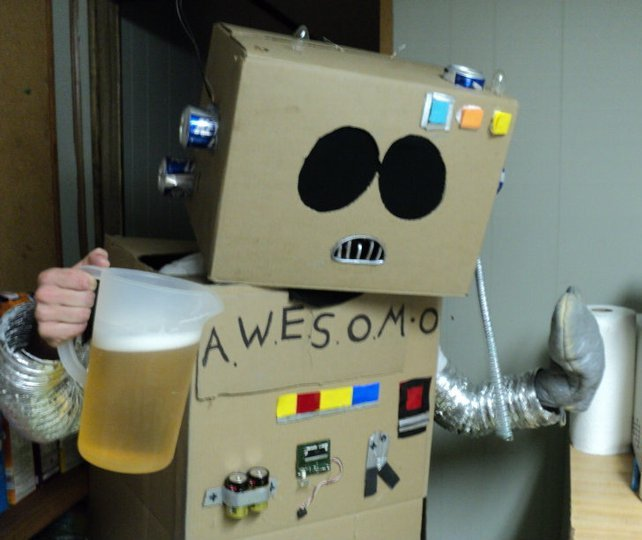
\includegraphics[width=60mm,totalheight=0.65\textheight]{figs/funny-drunk-guy-robot.jpg}
    \end{figure}
\end{frame}


\begin{frame}
  \frametitle{Fitting ICM to 3D IDM data: results (2)}
   \begin{figure}[h]
      \begin{tabular}{c c}
      %bla bla  & bla bla\\
      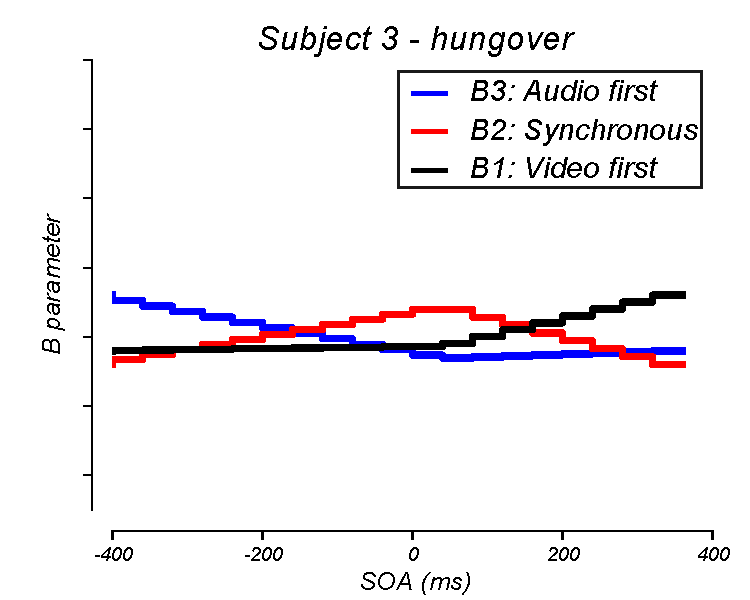
\includegraphics[width=50mm,totalheight=0.5\textheight]{figs/sub3_plot_Bs}
      &
      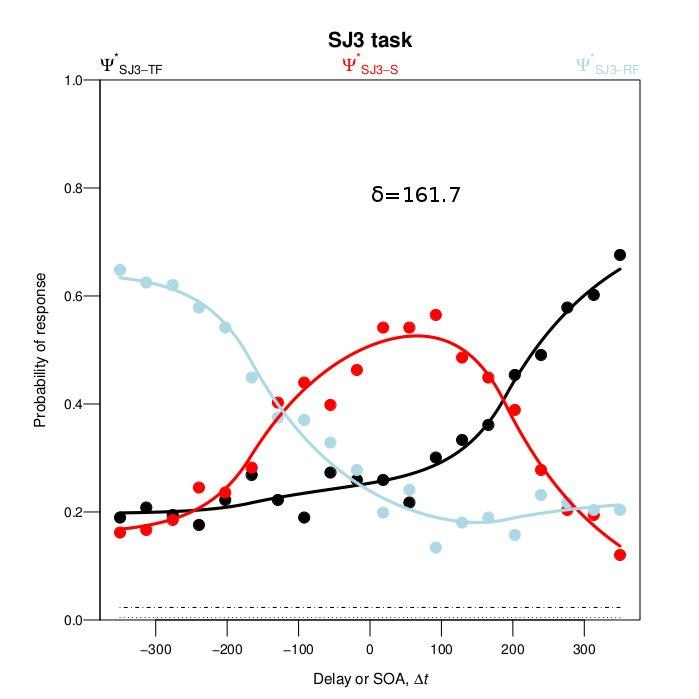
\includegraphics[width=50mm,totalheight=0.5\textheight]{figs/sub3_fitted_model.jpg}
       \end{tabular}
   \end{figure}
\end{frame}  


\begin{frame}
  \frametitle{Goal}
  \begin{columns}
  \begin{column}{0.30\textwidth}
  
\includegraphics[width=0.7\textwidth]{figs/checkbox-checked.png}
  \end{column}
  \begin{column}{0.70\textwidth}
  With an extended IDM model, simulate human behaviour in a three-alternative temporal judgment task
  \end{column}
  \end{columns}
  \begin{columns}
  \begin{column}{0.30\textwidth}
  
\includegraphics[width=0.7\textwidth]{figs/checkbox-checked.png}
  \end{column}
  \begin{column}{0.70\textwidth}
  Fit Independent-Channels Model (Miguel \& Rocio) to our simulated data 
  \end{column}
  \end{columns}
\end{frame} 


\begin{frame}
  \frametitle{Fitting ICM to 3D IDM data: results (3)}
  IDM simulated RT distribution for AF, S, and VF responses (\#Subject 2)
   \begin{figure}[h]
    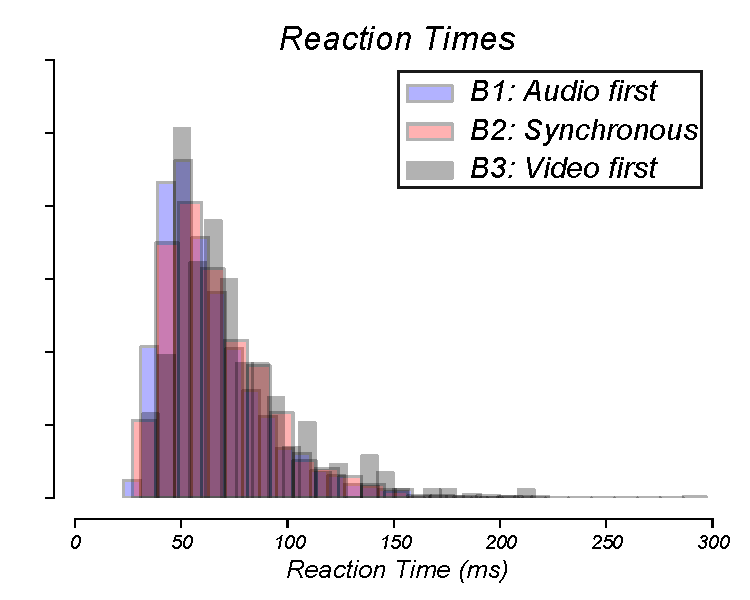
\includegraphics[width=60mm,totalheight=0.65\textheight]{figs/sub2_reaction_times2.pdf}
    \end{figure}
\end{frame}




%\begin{frame}
% \frametitle{Fitting IICM to 3D data: results 1}
%    \begin{equation}
%     f(d;\Delta t)=\big\{ 
%     \begin{array}{l l}
%      \small{\frac{\lambda_a\lambda_v}{{\lambda_a + \lambda_v}} \text{exp}[\lambda_v(d-\Delta t -\tau)]
%      & \quad \text{if} d\leq\Delta t +\tau \\
%      \small{\frac{\lambda_a\lambda_v}{{\lambda_a + \lambda_v}} \text{exp}}[-\lambda_a(d-\Delta t -\tau)] 
%      & \quad \text{if} d>\Delta t +\tau
%     \end{array}
%    \end{equation}
%\end{frame}    

\end{document}

